\hypertarget{_clip_8h}{
\section{Clip.h File Reference}
\label{_clip_8h}\index{Clip.h(123)@{Clip.h(123)}}
}


\subsection{Detailed Description}
Declaration of class \hyperlink{class_clip}{Clip}. 



Definition in file \hyperlink{_clip_8h-source}{Clip.h}.

{\tt \#include \char`\"{}NessieException.h\char`\"{}}\par
{\tt \#include \char`\"{}Pixel.h\char`\"{}}\par
{\tt \#include \char`\"{}Colorspace.h\char`\"{}}\par
{\tt \#include $<$Magick++.h$>$}\par
{\tt \#include $<$exception$>$}\par
{\tt \#include $<$iostream$>$}\par


Include dependency graph for Clip.h:\nopagebreak
\begin{figure}[H]
\begin{center}
\leavevmode
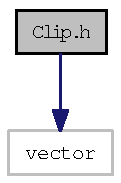
\includegraphics[width=212pt]{_clip_8h__incl}
\end{center}
\end{figure}


This graph shows which files directly or indirectly include this file:\nopagebreak
\begin{figure}[H]
\begin{center}
\leavevmode
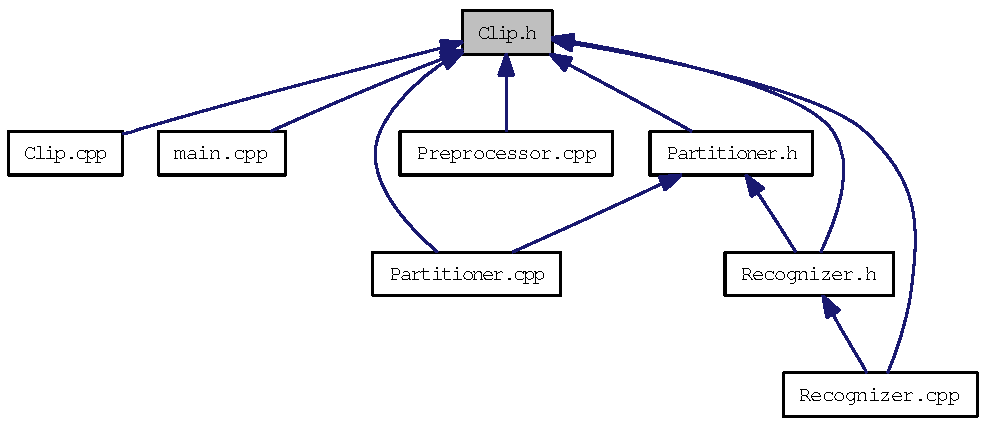
\includegraphics[width=215pt]{_clip_8h__dep__incl}
\end{center}
\end{figure}
\subsection*{Data Structures}
\begin{CompactItemize}
\item 
class \hyperlink{class_clip}{Clip}
\begin{CompactList}\small\item\em Press clip where the recognizer has to extract the text from. \item\end{CompactList}\end{CompactItemize}
